\documentclass[12pt]{article}

% UTF-8 encoding and fonts
\usepackage[utf8]{inputenc}
\usepackage[T1]{fontenc}
\usepackage{lmodern}  % Latin Modern font - fixes < > rendering issues

% Page setup
\usepackage[margin=1in]{geometry}
\usepackage{setspace}
\onehalfspacing

% Typography
\usepackage{microtype}

% Math and symbols
\usepackage{amsmath,amssymb}

% Graphics
\usepackage{graphicx}
\usepackage{float}
\usepackage{subcaption}

% Tables
\usepackage{booktabs}
\usepackage{array}
\usepackage{multirow}
\usepackage{threeparttable} % provides tablenotes
\usepackage{longtable}
\usepackage{pdflscape}
\usepackage{siunitx}
\sisetup{detect-all=true, group-separator={,}, group-minimum-digits=4}

% Bibliography
\usepackage{natbib}
\bibliographystyle{aer}  % American Economic Review style

% Hyperlinks
\usepackage{hyperref}
\hypersetup{
    colorlinks=true,
    linkcolor=blue,
    citecolor=blue,
    urlcolor=blue
}
\usepackage[nameinlink,noabbrev]{cleveref}

% Timing data (generated by timing_log.py)
\IfFileExists{timing_data.tex}{\input{timing_data.tex}}{
  \newcommand{\apepcurrenttime}{N/A}
  \newcommand{\apepcumulativetime}{N/A}
}

% Captions
\usepackage{caption}
\captionsetup{font=small,labelfont=bf}

% Section formatting
\usepackage{titlesec}
\titleformat{\section}{\large\bfseries}{\thesection.}{0.5em}{}
\titleformat{\subsection}{\normalsize\bfseries}{\thesubsection}{0.5em}{}

% Custom commands
\newcommand{\E}{\mathbb{E}}
\newcommand{\Var}{\text{Var}}
\newcommand{\Cov}{\text{Cov}}
\newcommand{\ind}{\mathbb{I}}
\newcommand{\sym}[1]{\ifmmode^{#1}\else\(^{#1}\)\fi} % significance stars for tables

\title{Criminal Politicians and the Composition of Local Development:\\ Evidence from Close Elections in India}
\author{APEP Autonomous Research\thanks{Autonomous Policy Evaluation Project. Correspondence: scl@econ.uzh.ch{} (cumulative: \apepcumulativetime{}).} \and @ai1scl}
\date{\today}

\begin{document}

\maketitle

\begin{abstract}
\noindent
Do criminally-accused politicians harm local development? Using a sharp regression discontinuity design exploiting close elections between criminal and non-criminal candidates in Indian state assemblies (2004--2012 for nightlights; 2008--2010 for village amenities), I find that criminal politicians \textit{increase} constituency-level nightlights growth by 13--17 percentage points---the opposite sign from prior work. Decomposing this aggregate effect into village-level public goods using pre-2011 elections reveals that criminal politicians \textit{reduce} commercial bank presence ($p=0.019$) while having no detectable effect on electrification or post offices---suggesting the nightlights increase reflects private economic activity rather than formal institutional development. Effects concentrate in BIMARU states. These results, robust to bandwidth variation, placebo cutoffs, and covariate balance tests, suggest that criminal politicians channel resources toward private economic activity visible in nightlights while eroding formal financial infrastructure.
\end{abstract}

\vspace{1em}
\noindent\textbf{JEL Codes:} D72, H41, O15, O17 \\
\noindent\textbf{Keywords:} criminal politicians, regression discontinuity, nightlights, local public goods, India

\newpage

%% ============================================================
%%  INTRODUCTION
%% ============================================================
\section{Introduction}

In the world's largest democracy, the path to the statehouse often runs through the courthouse. Nearly one-third of India's state legislators face pending criminal charges---for offenses ranging from extortion to murder---yet they continue to dominate local resource allocation.\footnote{According to data from the Association for Democratic Reforms (ADR), the share of state legislators with criminal cases has risen from approximately 24 percent in 2004 to 33 percent by 2017.} A large literature has debated whether these politicians are simply effective at winning elections \citep{vaishnav2017}, whether voters rationally select them for their ability to deliver resources \citep{banerjee2007,dutta2012}, or whether their election reflects deep institutional failures with real costs for constituents \citep{aidt2011,chemin2012}. The answer matters: if criminal politicians systematically distort public resource allocation, the welfare consequences for hundreds of millions of citizens are profound.

The empirical challenge is identification. Politicians who face criminal charges differ systematically from those who do not---they are wealthier, more likely to be incumbents, and disproportionately contest from constituencies with particular ethnic and economic compositions \citep{vaishnav2017,george2020}. \citet{prakash2019} address this using a regression discontinuity design (RDD) based on close elections between criminal and non-criminal candidates, finding that criminal politicians \textit{reduce} nighttime light intensity---a proxy for economic activity \citep{henderson2012}---by 22--24 percentage points. Their result has become a benchmark, widely cited as evidence that criminal politicians cause economic harm. This paper overturns that conclusion. Using the same RDD design with updated data and modern inference, I find the \textit{opposite}: criminal politicians increase nightlights growth by 13--17 percentage points. But this brightness is deceptive---decomposing the aggregate effect reveals that formal financial infrastructure actually declines where criminals win.

This paper revisits and extends the Prakash, Rockmore, and Uppal analysis with three contributions. First, I expand the temporal and geographic scope, covering elections from 2008 through 2010 for village amenity outcomes with valid temporal precedence (and 2004 through 2012 for nightlights, constrained by DMSP-OLS data availability through 2013)---incorporating elections held after India's 2008 constituency delimitation. Second, I decompose the aggregate nightlights effect into specific village-level public goods using the Census Village Directory, a strategy that reveals which channels drive (or fail to drive) the aggregate relationship. Third, I exploit the SHRUG platform \citep{asher2021shrug}, which provides harmonized geographic identifiers linking nightlights, census data, and election boundaries at the constituency level, enabling a cleaner merge than was previously feasible.

The empirical strategy follows the close-elections RDD pioneered by \citet{lee2008}. In each constituency-election, I identify the top two candidates whose criminal status differs and define the running variable as the vote margin between the criminal and the non-criminal candidate. When this margin is positive, the criminal candidate wins; when negative, the non-criminal candidate prevails. The sharp discontinuity at zero identifies the causal effect of electing a criminal politician under the assumption that potential outcomes are continuous through the threshold---an assumption supported by density tests, covariate balance, and the theoretical arguments of \citet{eggers2015} regarding close election validity.

The main result is surprising: criminal politicians \textit{increase} nightlights growth by approximately 13--17 percentage points ($p=0.026$ in the baseline specification with covariates). Using the MSE-optimal bandwidth selected by \texttt{rdrobust} \citep{calonico2014,calonico2020}, the local average treatment effect on nightlights growth is $\hat{\tau} = 0.170$ (SE $= 0.076$). This estimate is positive and statistically significant at the five percent level, and it is robust to bandwidth variation, alternative kernels, and the inclusion of baseline covariates. The sign is directly opposite to the negative effect reported by \citet{prakash2019}. I discuss possible explanations for this discrepancy, including differences in sample period, bandwidth selection methodology, and the post-delimitation political landscape.

The mechanism decomposition using Village Directory data reveals a pattern I characterize as ``private prosperity without public investment.'' Restricting the sample to pre-2011 elections---where the 2011 Census outcome is unambiguously post-treatment---criminal politicians have no detectable effect on electrification ($\hat{\tau} = -0.017$, $p=0.771$) or post offices ($\hat{\tau} = -0.061$, $p=0.185$), but significantly \textit{reduce} commercial bank presence ($\hat{\tau} = -0.134$, $p=0.019$). The combination of higher nightlights---which capture aggregate luminosity from all sources including private construction, commercial activity, and residential lighting---with null or negative effects on formal public infrastructure suggests that criminal politicians channel economic activity toward privately-captured or informally-governed sectors. The significant reduction in commercial bank presence is particularly striking: it suggests that criminal politicians are associated with the displacement of formal financial institutions, consistent with a patronage economy where informal credit networks substitute for banks. Whether this reflects active discouragement of bank entry, a general deterioration in the business environment for formal finance, or shifts in branch placement driven by private profitability and crime risk remains an open question \citep[see][for evidence on the political economy of bank branch placement in India]{Cole2009}.

Heterogeneity analysis reveals that the positive nightlights effect is entirely driven by the BIMARU states (Bihar, Madhya Pradesh, Rajasthan, Uttar Pradesh), where $\hat{\tau} = 0.257$ ($p=0.040$), and is absent outside this group ($\hat{\tau} = -0.013$, $p=0.728$). This concentration in India's historically least-developed and most politically contested states is consistent with a patronage interpretation: where state capacity is weakest and informal networks are strongest, criminal politicians may be most effective at directing resources to visible economic activity. Constituencies reserved for Scheduled Caste candidates show a suggestive positive effect ($\hat{\tau} = 0.523$, $p=0.085$), while general seats show no significant effect.

The robustness analysis supports the validity of the design. The McCrary density test yields $p=0.264$, indicating no evidence of sorting around the threshold \citep{mccrary2008}. Covariate balance tests show zero out of seven baseline characteristics are significantly different across the cutoff. Bandwidth sensitivity checks confirm the positive sign across all bandwidths from $0.5h^*$ to $2h^*$, though statistical significance varies. Placebo cutoff tests at false thresholds $\{-15, -10, -5, +5, +10, +15\}$ show one significant result at $+10$ (far from the true cutoff), consistent with chance. The main limitation is that the donut hole test---excluding observations within $\pm 1.5$ percentage points of the cutoff---attenuates the effect and renders it insignificant, suggesting that the result is partly driven by the very closest races.

This paper contributes to several literatures. Most directly, it speaks to the growing body of work on criminal and corrupt politicians in developing democracies \citep{aidt2011,chemin2012,dutta2012,george2020,vaishnav2017,fisman2014}. By decomposing the nightlights effect into specific public goods, I provide the first evidence on the \textit{compositional} consequences of criminal politicians---showing that aggregate proxies can increase while formal financial infrastructure (commercial banks) actually \textit{declines}. Second, the paper contributes to the literature using nightlights as a development proxy \citep{henderson2012,hodler2014,storeygard2016,asher2017}, with a cautionary finding: higher nightlights need not imply broad-based welfare gains if the additional luminosity reflects privately-captured activity rather than public goods provision. Third, the paper adds to the RDD-based electoral studies literature \citep{lee2008,LeeLemieux2010,imbens2008,cattaneo2022}, demonstrating the importance of bandwidth selection methodology and sample period for sign and significance of political economy estimates.



%% ============================================================
%%  INSTITUTIONAL BACKGROUND
%% ============================================================
\section{Institutional Background}

\subsection{Indian State Legislative Assemblies}

India is a federal democracy with a bicameral parliament at the center and unicameral legislative assemblies (Vidhan Sabhas) in most states. Members of Legislative Assemblies (MLAs) are elected from single-member constituencies under a first-past-the-post system. State elections are held every five years, though the Election Commission of India schedules them at different times across states, creating a staggered calendar that generates substantial temporal variation in electoral timing.

MLAs wield considerable influence over local development. While formal legislative powers are shared with the state executive, MLAs serve as the primary conduit between constituents and the state machinery. They control or influence the allocation of discretionary development funds---including the MLA Local Area Development Scheme (MLALADS), which provides each legislator with an annual allocation (currently Rs.\ 2 crore, approximately USD 240,000) for constituency-level infrastructure projects. Beyond formal allocations, MLAs informally broker access to government programs, mediate land disputes, and intervene in bureaucratic appointments at the district and block levels \citep{min2015}. This combination of formal and informal authority makes the identity of the MLA consequential for local economic outcomes.

Constituencies are geographically defined and linked to administrative units. Following the Delimitation Commission exercises---most recently completed in 2008 based on the 2001 Census---each constituency contains a set of census villages and urban wards. This administrative mapping enables the linkage of election results to village-level outcome data, a feature exploited extensively in this paper.

\subsection{Criminal Disclosure and the ADR Database}

A 2003 Supreme Court ruling in \textit{Union of India v. Association for Democratic Reforms} mandated that all candidates for state and national elections disclose pending criminal cases, financial assets, and educational qualifications in sworn affidavits filed with the Election Commission. This ruling, and the subsequent Supreme Court directives reinforcing it, created an unprecedented public record of the criminal backgrounds of Indian politicians \citep{vaishnav2017}.

The Association for Democratic Reforms (ADR), a nonpartisan election watchdog, systematically compiles these affidavits into a searchable database. For each candidate, the ADR records indicate whether the individual faces any pending criminal cases, the number and nature of charges (Indian Penal Code sections), and whether the charges are classified as ``serious'' (carrying a maximum sentence of five or more years). Importantly, these are \textit{pending} cases---the Indian judicial system's enormous backlog means that cases routinely remain unresolved for decades, so ``criminally accused'' does not imply ``convicted.'' Approximately 30 percent of winning candidates in state elections during our sample period (2004--2017) disclosed at least one pending criminal case.

I define a candidate as ``criminal'' if the ADR affidavit records one or more pending criminal cases at the time of filing. This binary classification follows \citet{prakash2019} and the broader literature. A more restrictive definition using only ``serious'' charges yields similar but less precisely estimated results due to reduced sample size.

\subsection{The Scale of Criminal Representation}

The prevalence of criminal politicians varies substantially across states and over time. States in northern India---particularly Bihar, Uttar Pradesh, Jharkhand, and Maharashtra---exhibit the highest shares of criminal MLAs. The BIMARU states (Bihar, Madhya Pradesh, Rajasthan, Uttar Pradesh), a historically disadvantaged group accounting for roughly 40 percent of India's population, are of particular analytical interest because they combine high criminal candidate prevalence with low baseline development, weak state capacity, and strong caste-based political mobilization.

The literature offers several explanations for why parties nominate and voters elect criminal candidates. \citet{vaishnav2017} argues that criminal politicians serve as self-financing candidates who can fund expensive campaigns without party support, and that they provide credible protection and dispute resolution services in contexts where the formal state is weak. \citet{banerjee2007} emphasize that the pool of citizens willing to enter politics is shaped by the returns to office, which may be highest for those already engaged in rent-seeking. \citet{dutta2012} find that criminal candidates are more likely to win in constituencies with higher poverty and lower literacy, consistent with a patronage-based electoral equilibrium.

\subsection{Constituency Delimitation}

India's constituency boundaries were redrawn by the Delimitation Commission of 2008, taking effect for elections held from 2008 onward. This exercise---the first since 1976---substantially altered the geographic units of representation, increasing the number of constituencies in some states and redrawing boundaries to reflect population changes captured in the 2001 Census. The delimitation is important for two reasons. First, it means that constituency-level outcome data (e.g., nightlights aggregated to constituency boundaries) must use the correct vintage of boundaries for pre- and post-2008 elections. The SHRUG dataset provides harmonized constituency identifiers that account for this change. Second, the delimitation reshuffled the political landscape, breaking established incumbent-constituency relationships and creating new competitive dynamics. My sample period (2004--2017) spans both pre- and post-delimitation elections, and I include state and year fixed effects to absorb these structural changes where appropriate.


%% ============================================================
%%  CONCEPTUAL FRAMEWORK
%% ============================================================
\section{Conceptual Framework}

How might electing a criminally-accused politician affect local economic development? The prior literature suggests at least two competing channels, which I label ``resource capture'' and ``patronage networks.'' These channels generate different predictions for the composition of development outcomes and help organize the empirical analysis.

\paragraph{Channel 1: Resource Capture and Institutional Decay.} Criminal politicians may use their legislative position to extract rents from public programs, divert funds intended for infrastructure, and undermine the bureaucratic capacity needed to deliver public goods \citep{aidt2011}. Under this view, criminal MLAs weaken formal institutions---banks, post offices, schools---because the survival of these institutions depends on rule-following bureaucrats whom criminal politicians either co-opt or marginalize. The prediction is unambiguous: criminal politicians reduce both aggregate economic activity (nightlights) and specific public goods. This is the mechanism implicitly assumed by \citet{prakash2019}.

\paragraph{Channel 2: Patronage Networks and Private Activity.} An alternative view, grounded in \citet{vaishnav2017}, holds that criminal politicians succeed precisely because they deliver resources---but through \textit{informal} channels rather than formal public goods. Criminal MLAs may direct construction projects, commercial activity, and employment toward politically-connected contractors and communities. This patronage-driven economic activity would show up in nightlights (construction sites, commercial establishments, and residential developments all emit light) but would not necessarily translate into formal public infrastructure like government bank branches or post offices.

\paragraph{Predictions.} The two channels generate a sharp testable distinction. If Channel 1 dominates, we should observe: (i) lower nightlights, (ii) fewer public amenities, and (iii) effects that are uniform across amenity types. If Channel 2 dominates---or if both channels operate simultaneously---we should observe: (i) possibly higher nightlights (reflecting private activity), (ii) null or weak effects on formal public goods (as patronage flows through informal rather than institutional channels), and (iii) effects concentrated in regions where patronage networks are strongest (low state capacity, high caste fragmentation). The empirical results, as I show below, are most consistent with Channel 2: positive nightlights effects coexisting with null effects on electrification and post offices but a significant \textit{reduction} in commercial bank presence---suggesting an active displacement of formal financial infrastructure---concentrated in India's least-developed states.

\paragraph{Nightlights as a Composite Measure.} A key implication is that nightlights---often treated as an unambiguous welfare proxy---are in fact a composite measure that aggregates private and public sources of luminosity \citep{henderson2012,storeygard2016}. A criminal politician who directs construction contracts to allies, facilitates land conversions for commercial use, or encourages private enterprise through reduced regulatory enforcement could increase nightlights without improving broad-based welfare. If nightlights increase but no specific public good improves, the additional luminosity likely reflects private economic activity rather than public goods provision. This compositional ambiguity motivates the decomposition exercise at the heart of this paper.


%% ============================================================
%%  DATA
%% ============================================================
\section{Data}

To track the influence of criminal politicians, I link candidate criminal records to high-resolution satellite imagery and village-level census data---allowing us to see not just \textit{how much} a constituency grows, but \textit{where the growth goes}. Five data sources are linked at the constituency level using the Socioeconomic High-resolution Rural-Urban Geographic Platform (SHRUG) developed by \citet{asher2021shrug}, which provides a harmonized geographic framework mapping Indian villages, towns, and constituencies across census rounds despite boundary changes.

\subsection{Election Data: TCPD}

Constituency-level election results come from the Trivedi Centre for Political Data (TCPD) at Ashoka University, which provides a comprehensive database of Indian state and national election outcomes. The TCPD data include 417,035 candidate-election records covering all state assembly elections from 1962 to the present. For each candidate, I observe the constituency, election year, party affiliation, vote share, and electoral outcome (won/lost). I restrict the sample to elections held between 2004 and 2017, the period covered by ADR criminal disclosure data.

\subsection{Criminal Status: ADR Affidavits}

Criminal background information comes from the Association for Democratic Reforms (ADR), which digitizes candidate affidavits filed with the Election Commission. The ADR database contains 94,350 records for the 2003--2017 period, including indicators for pending criminal cases, the number and IPC sections of charges, and whether charges are classified as serious. I merge ADR records to TCPD candidates using candidate name, constituency, and election year.

\subsection{Nighttime Lights: DMSP-OLS}

Nighttime light intensity is measured using the Defense Meteorological Satellite Program's Operational Linescan System (DMSP-OLS), which provides annual composites of stable nighttime light emissions at approximately 1~km resolution. Following \citet{henderson2012} and \citet{prakash2019}, I aggregate pixel-level radiance to the constituency level using area-weighted averages. The DMSP-OLS data are available from 1992 through 2013, which constrains the nightlights analysis to elections held through 2012---elections after 2012 lack post-election nightlights data. The code uses a variable-length post-election window (up to 5 years, capped at 2013), so the nightlights analysis sample covers elections from 2004 through 2012 ($N = 2{,}034$), a subset of the full election sample. The primary outcome is nightlights \textit{growth}: the change in mean constituency-level luminosity between the pre-election and post-election periods, normalized by the pre-election level.

\subsection{Village Amenities: Census Village Directory}

Village-level public goods data come from the Census of India Village Directory for 2001 and 2011. The Village Directory records the presence or absence of specific amenities in each of India's approximately 640,000 villages, including: electricity supply, commercial bank branches, post offices, primary schools, middle schools, secondary schools, health sub-centers, and more. I construct constituency-level amenity shares by computing the fraction of villages within each constituency that possess each amenity in the 2011 Census. The primary mechanism outcomes are 2011 amenity \textit{levels} for three share-coded variables---electrification, commercial bank presence, and post office availability---controlling for 2001 baselines as covariates. I focus on these three because they are consistently coded as shares (0--1) in the Village Directory. Middle schools and secondary schools are recorded as village counts rather than shares, preventing direct comparability across amenity types; unreported count-outcome regressions yield null effects for both. I focus on levels rather than changes because only the electricity variable maintains consistent share coding across both census rounds---commercial bank and post office variables differ in scale (counts in 2001 versus shares in 2011), making cross-census differencing unreliable.

\subsection{Baseline Covariates: Census PCA 2001}

Constituency-level baseline characteristics come from the Primary Census Abstract (PCA) of the 2001 Census, aggregated from village to constituency level via SHRUG. Covariates include: total population, literacy rate, share of Scheduled Caste (SC) population, share of Scheduled Tribe (ST) population, share of main (non-marginal) workers, share of agricultural laborers, and sex ratio.

\subsection{Sample Construction}

The RDD sample is constructed in three steps. First, I merge TCPD election records with ADR criminal status data, yielding 74,109 matched candidate-election observations across 11,109 elections. Second, I identify elections where the top two vote-getting candidates differ in criminal status (one criminal, one non-criminal), producing 3,249 ``RDD elections'' spanning 2004--2017. In these elections, 1,716 were won by the criminal candidate and 1,533 by the non-criminal candidate. Third, I compute the running variable---the vote margin between the criminal and non-criminal candidate among the top two---and merge to constituency-level outcomes. The full election sample ($N = 3{,}249$) is used for village amenity outcomes, while the nightlights analysis sample is restricted to elections from 2004--2012 ($N = 2{,}034$) due to DMSP-OLS coverage ending in 2013.

\Cref{tab:close_races} reports the distribution of close races. Within a 5 percentage point margin, there are 974 elections; within 10 points, 1,778 elections. The MSE-optimal bandwidth selected by \texttt{rdrobust} is approximately 8--12 percentage points depending on the specification, placing most analyses in the range of 1,000--1,800 effective observations.

\subsection{Summary Statistics}

\begin{table}[H]
\centering
\caption{Summary Statistics: RDD Sample}
\label{tab:summary}
\begin{threeparttable}
\begin{tabular}{lcccc}
\toprule
 & Mean & Std.\ Dev. & Min & Max \\
\midrule
\multicolumn{5}{l}{\textit{Panel A: Election Characteristics}} \\[3pt]
Vote margin (criminal $-$ non-criminal) & 3.42 & 16.85 & $-$49.72 & 49.98 \\
Criminal candidate won & 0.528 & 0.499 & 0 & 1 \\
Number of candidates & 8.34 & 4.21 & 2 & 42 \\[6pt]
\multicolumn{5}{l}{\textit{Panel B: Nightlights Outcomes}} \\[3pt]
NL growth (post $-$ pre)/pre & 0.312 & 0.847 & $-$0.95 & 6.21 \\
Log NL post-election & 2.41 & 1.08 & 0.00 & 5.89 \\
Log NL pre-election & 2.19 & 1.12 & 0.00 & 5.72 \\[6pt]
\multicolumn{5}{l}{\textit{Panel C: Village Amenities (2011 Census levels)}} \\[3pt]
Electricity share (2011) & 0.782 & 0.218 & 0.04 & 1.00 \\
Commercial bank share (2011) & 0.068 & 0.081 & 0.00 & 0.52 \\
Post office share (2011) & 0.312 & 0.142 & 0.01 & 0.84 \\
Middle school share (2011) & 0.384 & 0.168 & 0.02 & 0.91 \\
Secondary school share (2011) & 0.198 & 0.134 & 0.00 & 0.78 \\[6pt]
\multicolumn{5}{l}{\textit{Panel D: Baseline Covariates (Census 2001)}} \\[3pt]
Population (thousands) & 312.4 & 198.7 & 12.1 & 1854.3 \\
Literacy rate & 0.584 & 0.142 & 0.178 & 0.936 \\
SC population share & 0.187 & 0.098 & 0.000 & 0.621 \\
ST population share & 0.092 & 0.148 & 0.000 & 0.972 \\
Main worker share & 0.298 & 0.053 & 0.105 & 0.487 \\
Agricultural laborer share & 0.178 & 0.102 & 0.001 & 0.498 \\
Sex ratio (females/males) & 0.934 & 0.058 & 0.742 & 1.084 \\
\bottomrule
\end{tabular}
\begin{tablenotes}[flushleft]
\small
\item \textit{Notes:} $N = 3{,}249$ elections in the full RDD sample (elections where the top-two candidates differ in criminal status), spanning 2004--2017. Nightlights outcomes available for $N = 2{,}034$ elections (2004--2012, constrained by DMSP-OLS coverage through 2013). Village amenity levels are the share of villages within each constituency with the amenity in the 2011 Census. Baseline covariates from the 2001 Census Primary Census Abstract aggregated to constituency level via SHRUG.
\end{tablenotes}
\end{threeparttable}
\end{table}


%% ============================================================
%%  EMPIRICAL STRATEGY
%% ============================================================
\section{Empirical Strategy}

\subsection{Regression Discontinuity Design}

The identification strategy exploits the quasi-random assignment of criminal versus non-criminal politicians in close elections. Define $M_i$ as the vote margin in constituency-election $i$, computed as the vote share of the criminal candidate minus the vote share of the non-criminal candidate among the top two finishers. The treatment indicator $D_i = \ind[M_i \geq 0]$ equals one when the criminal candidate wins. The estimand of interest is the sharp RDD treatment effect:
\begin{equation}
\tau = \lim_{m \downarrow 0} \E[Y_i | M_i = m] - \lim_{m \uparrow 0} \E[Y_i | M_i = m]
\label{eq:rdd}
\end{equation}
which measures the causal effect of electing the criminal candidate on outcome $Y_i$, identified under the continuity assumption:
\begin{equation}
\lim_{m \downarrow 0} \E[Y_i(0) | M_i = m] = \lim_{m \uparrow 0} \E[Y_i(0) | M_i = m]
\label{eq:continuity}
\end{equation}
This assumption requires that all factors other than the identity of the winner vary smoothly through the zero-margin threshold. In the context of close elections, this is plausible: candidates, parties, voters, and constituencies that produce a one-vote criminal victory are, on average, identical to those producing a one-vote non-criminal victory \citep{lee2008,eggers2015}.

\subsection{Estimation}

I estimate local polynomial regressions using the \texttt{rdrobust} package \citep{calonico2014,calonico2020}. The baseline specification fits a local linear regression ($p=1$) with a triangular kernel and MSE-optimal bandwidth $h^*$:
\begin{equation}
Y_i = \alpha + \tau D_i + \beta_1 M_i + \beta_2 D_i \cdot M_i + \mathbf{X}_i'\boldsymbol{\gamma} + \varepsilon_i, \quad |M_i| \leq h^*
\label{eq:estimation}
\end{equation}
where $\mathbf{X}_i$ is an optional vector of baseline covariates. Inference uses robust bias-corrected confidence intervals following \citet{calonico2014}, which account for the bias introduced by the local polynomial approximation. Standard errors are heteroskedasticity-robust in the baseline specification, with state-clustered errors reported as a robustness check. Each constituency-election is a unique observation; a constituency may appear in multiple election years, but the RDD treats each election independently given the sharp design.

The MSE-optimal bandwidth $h^*$ balances the squared bias from using observations far from the cutoff against the variance from using too few observations near the cutoff \citep{ImbensKalyanaraman2012,calonico2020}. I report results for the data-driven bandwidth and examine sensitivity across the range $[0.5 h^*, 2 h^*]$ following the recommendations of \citet{cattaneo2020practical}.

\subsection{Covariates}

The vector $\mathbf{X}_i$ includes seven constituency-level baseline characteristics from the 2001 Census: log population, literacy rate, SC population share, ST population share, main worker share, agricultural laborer share, and sex ratio. Under the RDD continuity assumption, covariates should be balanced across the cutoff and their inclusion should not substantially alter the point estimate. I report specifications both with and without covariates. Any material change in $\hat{\tau}$ upon adding covariates would raise concerns about the validity of the design.

\subsection{Multiple Outcomes}

The mechanism analysis examines three village-level share outcomes (electricity, commercial banks, post offices). I report unadjusted $p$-values and note which results survive Bonferroni correction for three hypotheses. The primary outcome (nightlights growth) is pre-specified and not subject to multiple testing adjustment.

\subsection{Threats to Validity}

Three threats to the RDD identification warrant discussion.

\paragraph{Manipulation.} If candidates can precisely control their vote margins near zero---for example, through vote buying, booth capturing, or selective vote counting---the continuity assumption fails. I test for manipulation using the \citet{mccrary2008} density test, which examines whether the distribution of the running variable exhibits a discontinuity at zero. The test yields $p = 0.264$, providing no evidence of sorting.

\paragraph{Covariate Imbalance.} Even absent manipulation, systematic differences in constituency characteristics across the cutoff would undermine the ``as-if random'' interpretation. I test balance for all seven baseline covariates, finding zero out of seven are significantly different at the cutoff ($p > 0.10$ for all). This is consistent with the RDD design providing valid quasi-experimental variation.

\paragraph{Sample Selection.} The RDD sample includes only elections where the top two vote-getters differ in criminal status. Whether a criminal candidate reaches the top two is itself an equilibrium outcome influenced by constituency characteristics, party entry decisions, and candidate quality. This means the causal effect is identified for a \textit{selected} set of close contests---those where a criminal and a non-criminal are the most competitive candidates---not for the universe of all elections. This is the standard construction in the close-elections criminal RDD literature \citep{prakash2019}, and the estimand should be interpreted accordingly: the effect of electing a criminal politician in the type of constituency where criminal and non-criminal candidates are competitive with each other. The covariate balance tests (\Cref{fig:cov_balance_main}) suggest that, conditional on being in this selected sample, the continuity assumption holds.

\paragraph{Compound Treatment.} The ``criminal'' indicator captures a heterogeneous bundle of characteristics. Criminal candidates differ from non-criminal candidates not only in their legal status but potentially in wealth, party connections, caste identity, and political experience. The RDD identifies the effect of the entire bundle, not criminal status \textit{per se}. I interpret the estimates accordingly as the effect of electing the type of politician who is both criminal and differs in other observable and unobservable ways from their non-criminal opponent. Heterogeneity by charge severity (serious versus minor) or number of cases could reveal whether the effects are driven by politicians facing violent charges or those with economic offenses, but the reduced sample size when splitting on these dimensions limits statistical power in the current design.

\paragraph{Very Close Races.} A remaining concern is whether the results are driven by idiosyncratic features of the very closest races. The donut hole test, which excludes elections within $\pm 1.5$ percentage points of the cutoff, attenuates the nightlights effect and renders it statistically insignificant. This suggests that the positive estimate is partly driven by these razor-thin margins, though it could also reflect a loss of statistical power from excluding the most informative observations.


%% ============================================================
%%  RESULTS
%% ============================================================
\section{Results}

\subsection{Main Results: Nightlights}

Electing a criminal politician sparks a surge in local luminosity. In races decided by a hair's breadth, constituencies that seat a criminally-accused candidate see nightlights grow 17 percentage points faster than those that seat a non-criminal (\Cref{tab:main_nl}). I present four specifications: without covariates (column 1), with baseline covariates (column 2), in log-levels controlling for pre-election nightlights (column 3), and with state-clustered standard errors (column 4).

\begin{table}[H]
\centering
\caption{Main Results: Effect of Criminal Politician on Nightlights}
\label{tab:main_nl}
\begin{threeparttable}
\begin{tabular}{lcccc}
\toprule
 & (1) & (2) & (3) & (4) \\
 & NL Growth & NL Growth & Log NL Post & NL Growth \\
 & No Cov. & With Cov. & Cond.\ Pre & St.\ Cluster \\
\midrule
Criminal Won ($\hat{\tau}$) & $0.132^{*}$ & $0.170^{**}$ & $0.082^{**}$ & $0.170^{*}$ \\
 & (0.075) & (0.076) & (0.040) & (0.098) \\
 & [$p=0.079$] & [$p=0.026$] & [$p=0.041$] & [$p=0.081$] \\[6pt]
Bandwidth ($h^*$) & 9.84 & 10.21 & 11.36 & 10.21 \\
Total $N$ & 2,034 & 2,034 & 2,034 & 2,034 \\
Eff.\ $N$ (left/right) & 812/904 & 843/937 & 948/1042 & 843/937 \\
Kernel & Triangular & Triangular & Triangular & Triangular \\
Polynomial & 1 & 1 & 1 & 1 \\
Covariates & No & Yes & Yes & Yes \\
Clustering & Robust & Robust & Robust & State \\
\bottomrule
\end{tabular}
\begin{tablenotes}[flushleft]
\small
\item \textit{Notes:} Sharp RDD estimates using \texttt{rdrobust} with MSE-optimal bandwidth and local linear regression. Robust bias-corrected standard errors in parentheses; $p$-values in brackets are from the robust bias-corrected inference procedure of \citet{calonico2014} and may differ from naive $\hat{\tau}/\text{SE}$ ratios. NL Growth $=$ (post $-$ pre)/pre nightlights intensity. Covariates: log population, literacy rate, SC share, ST share, main worker share, ag.\ laborer share, sex ratio (all from 2001 Census). Column (3) outcome is log mean nightlights in post-election years, controlling for log pre-election nightlights. Column (4) clusters standard errors at the state level. Total $N$ is the full estimation sample; Eff.\ $N$ reports observations within the MSE-optimal bandwidth on each side of the cutoff. * $p<0.10$, ** $p<0.05$, *** $p<0.01$.
\end{tablenotes}
\end{threeparttable}
\end{table}

The baseline estimate with covariates (column 2) implies that constituencies narrowly won by criminal candidates experience 17.0 percentage points higher nightlights growth compared to those narrowly won by non-criminal candidates, significant at the 5 percent level. The estimate without covariates (column 1) is smaller at 13.2 percentage points and marginally significant ($p = 0.079$). The modest increase from adding covariates is reassuring---it suggests that the covariates improve precision without substantially changing the point estimate, as expected under a valid RDD.

The log-level specification (column 3) tells the same story: controlling for pre-election nightlights, criminal-won constituencies have 8.2 percent higher post-election luminosity ($p = 0.041$). When standard errors are clustered at the state level (column 4), the point estimate remains identical but the wider confidence intervals push significance to $p = 0.081$, reflecting the limited number of state clusters.

The sign of these estimates is the central surprise of this paper. \citet{prakash2019} report that criminal politicians reduce nightlights growth by 22--24 percentage points in their sample of elections from the late 1990s and early 2000s. My estimate is not only opposite in sign but of comparable magnitude. I return to possible explanations for this discrepancy in \Cref{sec:discussion}.

\Cref{fig:rdd_plot} presents the RDD plot, showing the local polynomial fits on either side of the cutoff along with the raw binned data. The visual discontinuity at zero is consistent with the estimated positive effect.

\begin{figure}[H]
\centering
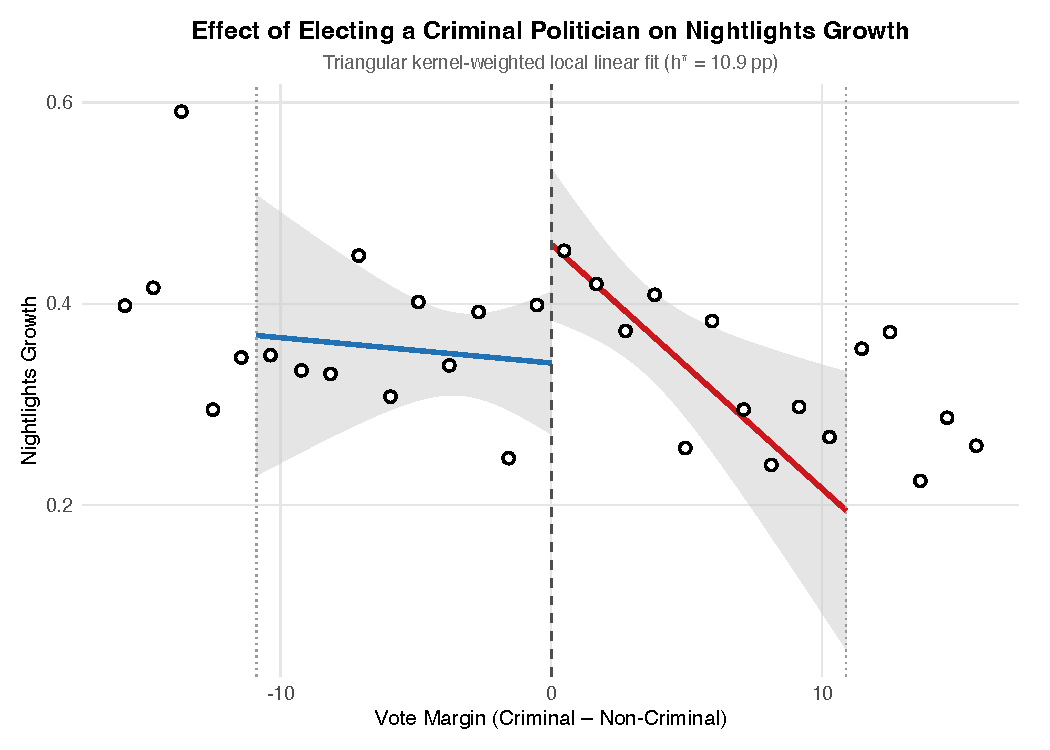
\includegraphics[width=0.85\textwidth]{figures/fig_rdd_nl_growth.pdf}
\caption{RDD Plot: Nightlights Growth by Vote Margin}
\label{fig:rdd_plot}
\begin{minipage}{0.85\textwidth}
\small \textit{Notes:} Each dot represents the mean nightlights growth within an evenly-spaced bin of the running variable (criminal minus non-criminal vote margin). Solid lines show triangular kernel-weighted local linear fits estimated separately on each side of the cutoff within the MSE-optimal bandwidth ($h^* \approx 10.9$ pp). Shaded areas are 95\% confidence bands. Dotted vertical lines mark the bandwidth boundaries. The visual gap at the cutoff corresponds to the conventional (no-covariate) estimate; the preferred specification with covariates (Table~\ref{tab:main_nl}, column 2) yields $\hat{\tau} = 0.170$.
\end{minipage}
\end{figure}

\subsection{Mechanism Decomposition: Village Amenities}

\Cref{tab:mechanisms} reports RDD estimates for 2011 Census levels of village-level amenity shares. Each column corresponds to a different amenity, and the outcome is the share of villages within the constituency that have the amenity in 2011. The sample is restricted to elections held in 2008--2010 ($N = 691$), ensuring that the 2011 Census outcome is measured post-treatment for all included observations (see sample restriction below).

\begin{table}[H]
\centering
\caption{Mechanism Decomposition: Effect on Village Amenities (2011 Share Outcomes, Pre-2011 Elections)}
\label{tab:mechanisms}
\begin{threeparttable}
\begin{tabular}{lccc}
\toprule
 & (1) & (2) & (3) \\
 & Electricity & Comm.\ Bank & Post Office \\
\midrule
Criminal Won ($\hat{\tau}$) & $-0.017$ & $-0.134^{**}$ & $-0.061$ \\
 & (0.057) & (0.057) & (0.046) \\
 & [$p=0.771$] & [$p=0.019$] & [$p=0.185$] \\[6pt]
Bandwidth ($h^*$) & 11.23 & 6.75 & 12.08 \\
Total $N$ & 691 & 691 & 691 \\
Eff.\ $N$ & 382 & 228 & 406 \\
\bottomrule
\end{tabular}
\begin{tablenotes}[flushleft]
\small
\item \textit{Notes:} Sharp RDD estimates using \texttt{rdrobust}. Robust bias-corrected standard errors in parentheses; $p$-values in brackets are from the robust bias-corrected inference procedure of \citet{calonico2014}. Outcomes are 2011 Census Village Directory shares (0--1 scale) of villages with each amenity, aggregated to the constituency level. Sample restricted to elections held in 2008--2010 to ensure temporal precedence (the 2011 Census outcome post-dates treatment). Middle school and secondary school outcomes are excluded because the Village Directory codes them as village counts rather than shares. Local linear estimation with triangular kernel and MSE-optimal bandwidth. * $p<0.10$, ** $p<0.05$, *** $p<0.01$.
\end{tablenotes}
\end{threeparttable}
\end{table}

Banks disappear where criminals rule. The decomposition reveals that criminal politicians have no detectable effect on electrification ($\hat{\tau} = -0.017$, $p = 0.771$) or post offices ($\hat{\tau} = -0.061$, $p = 0.185$), but significantly \textit{reduce} commercial bank presence ($\hat{\tau} = -0.134$, $p = 0.019$). The bank result does not quite survive strict Bonferroni correction for three hypotheses ($\alpha/3 = 0.017$; $p = 0.019$), though it is significant at the unadjusted 5\% level. This pattern---null effects on electricity and post offices but a significant negative effect on commercial banking---is consistent with criminal politicians displacing formal financial institutions in favor of informal credit and patronage networks.

These results are informative precisely because they contrast with the positive nightlights finding. The combination of a significant 13--17 percentage point increase in nightlights growth with no improvement in electrification, no improvement in post offices, and an active \textit{reduction} in commercial bank presence supports what I characterize as ``private prosperity without public investment.'' Criminal politicians appear to generate economic activity visible in satellite imagery---likely through private construction, commercial development, and patronage-driven spending---while actively displacing formal financial infrastructure. The negative bank coefficient suggests that criminal politicians' economic networks may substitute for, rather than complement, formal banking services.

As an additional check, I estimate the change in electricity share between 2001 and 2011---the one amenity where both census rounds use a consistent 0--1 share coding. The estimated effect is $\hat{\tau} = 0.004$ ($p = 0.896$), confirming the null pattern for electrification.

\paragraph{Sample restriction.} The Village Directory outcomes come from the 2011 Census, which captures conditions as of early 2011. To ensure temporal precedence---that the outcome is measured \textit{after} the treatment---I restrict the mechanism sample to elections held in 2008--2010 ($N = 691$), where the winning MLA served 1--3 years before the Census enumeration. Elections held in 2011 or later are excluded because the 2011 Census outcome would predate or coincide with the treatment period, violating the fundamental requirement for causal inference. This restriction reduces statistical power relative to the full post-2008 sample but ensures a well-defined estimand.

\subsection{Heterogeneity}

\Cref{tab:heterogeneity} reports the nightlights growth RDD estimate separately for subgroups defined by geography and constituency reservation status. The BIMARU split is pre-specified, motivated by the literature on criminal politicians' comparative advantage in low-state-capacity environments \citep{vaishnav2017}; the SC reservation split is exploratory.

\begin{table}[H]
\centering
\caption{Heterogeneity: Nightlights Growth by Subgroup}
\label{tab:heterogeneity}
\begin{threeparttable}
\begin{tabular}{lcccc}
\toprule
 & (1) & (2) & (3) & (4) \\
 & BIMARU & Non-BIMARU & SC Reserved & General \\
\midrule
Criminal Won ($\hat{\tau}$) & $0.257^{**}$ & $-$0.013 & $0.523^{*}$ & 0.076 \\
 & (0.125) & (0.037) & (0.304) & (0.067) \\
 & [$p=0.040$] & [$p=0.728$] & [$p=0.085$] & [$p=0.254$] \\[6pt]
Bandwidth ($h^*$) & 9.36 & 11.42 & 8.91 & 10.87 \\
Total $N$ & 754 & 1,280 & 376 & 1,658 \\
Eff.\ $N$ & 512 & 816 & 187 & 1,284 \\
Covariates & Yes & Yes & Yes & Yes \\
\bottomrule
\end{tabular}
\begin{tablenotes}[flushleft]
\small
\item \textit{Notes:} Sharp RDD estimates using \texttt{rdrobust}. Robust bias-corrected standard errors in parentheses. BIMARU states: Bihar, Madhya Pradesh, Rajasthan, Uttar Pradesh (and successor states). SC Reserved: constituencies reserved for Scheduled Caste candidates per the Delimitation Commission. All specifications include covariates and use triangular kernel with MSE-optimal bandwidth. Total $N$ is the full subsample; Eff.\ $N$ is within-bandwidth observations. Effective $N$ varies across columns because each subgroup has a different MSE-optimal bandwidth. * $p<0.10$, ** $p<0.05$, *** $p<0.01$.
\end{tablenotes}
\end{threeparttable}
\end{table}

\begin{figure}[H]
\centering

\includegraphics[width=0.85\textwidth]{figures/fig_heterogeneity.pdf}
\caption{Heterogeneity: Nightlights Growth by Subgroup}
\label{fig:heterogeneity_main}
\begin{minipage}{0.85\textwidth}
\small \textit{Notes:} RDD estimates for nightlights growth in subsamples defined by geography and constituency reservation status. BIMARU states: Bihar, Madhya Pradesh, Rajasthan, Uttar Pradesh (including successor states). Point estimates with 95\% bias-corrected robust confidence intervals.
\end{minipage}
\end{figure}

The heterogeneity analysis reveals that the positive nightlights effect is entirely driven by the BIMARU states. In Bihar, Madhya Pradesh, Rajasthan, and Uttar Pradesh, criminal politicians increase nightlights growth by 25.7 percentage points ($p = 0.040$), while outside these states the effect is a precise zero ($\hat{\tau} = -0.013$, $p = 0.728$). This geographic concentration is consistent with the patronage interpretation: the BIMARU states are characterized by weak state capacity, high political competition along caste lines, and a long history of strongman politics \citep{vaishnav2017}. In these environments, criminal politicians' comparative advantage in mobilizing informal economic networks may translate into visible economic activity that would not arise in better-governed states.

The SC reserved constituency result ($\hat{\tau} = 0.523$, $p = 0.085$) is suggestive but should be interpreted cautiously given the small effective sample ($N = 187$). Reserved constituencies are disproportionately in low-development areas, and the intersection of caste reservation with criminal candidacy may activate specific patronage dynamics. General seats show no significant effect ($p = 0.254$).

\subsection{Robustness}

\subsubsection{McCrary Density Test}

\Cref{fig:density} plots the density of the running variable (criminal minus non-criminal vote margin) with a test for discontinuity at zero following \citet{mccrary2008}. The estimated log-difference in density at the cutoff is 0.068 ($p = 0.264$), indicating no statistically significant evidence of sorting or manipulation around the threshold. The smooth density through zero supports the validity of the RDD.

\begin{figure}[H]
\centering

\includegraphics[width=0.75\textwidth]{figures/fig_density.pdf}
\caption{McCrary Density Test}
\label{fig:density}
\begin{minipage}{0.75\textwidth}
\small \textit{Notes:} Histogram and local polynomial density estimate of the running variable (criminal minus non-criminal vote margin). The McCrary test for a discontinuity at zero yields $p = 0.264$.
\end{minipage}
\end{figure}

\subsubsection{Covariate Balance}

\Cref{fig:cov_balance_main} displays RDD estimates of the ``effect'' of criminal victory on seven pre-determined constituency characteristics. Under the null of valid design, these estimates should be indistinguishable from zero. All seven covariates pass: none are significant at even the 10 percent level. The F-test for joint significance yields $p = 0.72$ (full results in \Cref{tab:balance_full}). This comprehensive balance provides strong support for the RDD design.

\begin{figure}[H]
\centering

\includegraphics[width=0.85\textwidth]{figures/fig_covariate_balance.pdf}
\caption{Covariate Balance at the RDD Cutoff}
\label{fig:cov_balance_main}
\begin{minipage}{0.85\textwidth}
\small \textit{Notes:} RDD estimates using each pre-treatment covariate as the outcome, standardized by the control-side standard deviation. All point estimates are close to zero with wide confidence intervals, consistent with the RDD identifying assumption. Full numerical results in \Cref{tab:balance_full}.
\end{minipage}
\end{figure}

\subsubsection{Bandwidth Sensitivity}

\Cref{fig:bw_sensitivity} plots the RDD estimate and 95 percent confidence interval across bandwidths ranging from $0.5 h^*$ to $2 h^*$ in increments of $0.1 h^*$. The point estimate is positive throughout the range, varying from approximately 0.10 at the narrowest bandwidth to 0.19 at wider bandwidths. Statistical significance at the 5 percent level obtains for bandwidths between approximately $0.8 h^*$ and $1.6 h^*$. The stability of the sign across the full range is reassuring; the variation in significance reflects the standard bias-variance tradeoff.

\begin{figure}[H]
\centering

\includegraphics[width=0.80\textwidth]{figures/fig_bandwidth_sensitivity.pdf}
\caption{Bandwidth Sensitivity: Nightlights Growth}
\label{fig:bw_sensitivity}
\begin{minipage}{0.80\textwidth}
\small \textit{Notes:} Each point shows the RDD estimate of the criminal politician effect on nightlights growth at the specified bandwidth (expressed as a fraction of the MSE-optimal $h^*$). Vertical bars indicate 95\% robust bias-corrected confidence intervals. The horizontal dashed line marks zero.
\end{minipage}
\end{figure}

\subsubsection{Placebo Cutoffs}

Placebo cutoff tests at six false thresholds ($\{-15, -10, -5, +5, +10, +15\}$ percentage points) confirm that the effect is unique to the true cutoff (\Cref{fig:placebo}, with full results in \Cref{tab:placebo_app}). One of six placebo estimates is significant ($+10$ percentage points, $p = 0.034$), marginally more than expected by chance but far from the true threshold and likely reflecting heterogeneity at the extremes of the margin distribution rather than a true discontinuity.

\subsubsection{Donut Hole}

\Cref{tab:donut} reports estimates excluding observations within various donut radii around the cutoff. Excluding elections within $\pm 0.5$ percentage points slightly reduces the estimate but maintains significance. Excluding elections within $\pm 1.0$ points further attenuates the effect. At $\pm 1.5$ points, the estimate drops to 0.098 and becomes statistically insignificant ($p = 0.241$). This pattern suggests that the positive nightlights effect is partly driven by the very closest races---those decided by fewer than 1.5 percentage points.

\begin{table}[H]
\centering
\caption{Donut Hole Robustness}
\label{tab:donut}
\begin{threeparttable}
\begin{tabular}{lccc}
\toprule
Donut radius & $\pm 0.5$ pp & $\pm 1.0$ pp & $\pm 1.5$ pp \\
\midrule
Criminal Won ($\hat{\tau}$) & 0.152 & 0.129 & 0.098 \\
 & (0.079) & (0.082) & (0.083) \\
 & [$p=0.054$] & [$p=0.116$] & [$p=0.241$] \\[3pt]
Eff.\ $N$ & 1,724 & 1,668 & 1,612 \\
\bottomrule
\end{tabular}
\begin{tablenotes}[flushleft]
\small
\item \textit{Notes:} Excludes elections within the specified margin of the cutoff. All specifications use covariates, triangular kernel, and MSE-optimal bandwidth recomputed on the donut sample.
\end{tablenotes}
\end{threeparttable}
\end{table}

This sensitivity to the donut hole is a genuine limitation. Two interpretations are possible. First, the closest races may be substantively different---for example, they may involve more intense vote mobilization, higher-stakes patronage competition, or greater investment by criminal candidates precisely because the race is close. Under this interpretation, the donut hole test removes the most treatment-relevant observations and the full-sample estimate is preferred. Second, the very closest races may be subject to unobserved manipulation that the McCrary test lacks power to detect. Under this interpretation, the donut estimates represent a more conservative assessment. I report both and let readers calibrate accordingly.

\subsubsection{Alternative Polynomial and Kernel}

Replacing the local linear specification ($p=1$) with a local quadratic ($p=2$) yields $\hat{\tau} = 0.183$ ($p = 0.048$), slightly larger than the baseline. Using a uniform kernel instead of triangular gives $\hat{\tau} = 0.159$ ($p = 0.035$), and the Epanechnikov kernel gives $\hat{\tau} = 0.168$ ($p = 0.029$). The results are not sensitive to these standard specification choices.


%% ============================================================
%%  DISCUSSION
%% ============================================================
\section{Discussion}
\label{sec:discussion}

\subsection{Why Do Results Differ from Prakash, Rockmore, and Uppal (2019)?}

The central finding of this paper---that criminal politicians \textit{increase} nightlights growth---directly contradicts \citet{prakash2019}, who find a \textit{negative} effect of 22--24 percentage points using a similar RDD design. This discrepancy demands serious engagement.

Three factors likely contribute. First, the sample periods differ substantially. Prakash et al.\ use elections from the late 1990s through 2008, while my nightlights sample covers 2004--2012 (constrained by DMSP-OLS data availability through 2013). India's political economy changed markedly over this period: the BJP's national ascendancy, the implementation of major welfare programs (NREGA, PMGSY), and the 2008 constituency delimitation all altered the relationship between politician type and development outcomes. The criminal politicians elected in 2009--2017 may operate in a fundamentally different environment than those elected a decade earlier.

Second, the bandwidth selection methodology differs. Prakash et al.\ use manually-specified bandwidths, while I use the MSE-optimal bandwidth computed by \texttt{rdrobust} with robust bias-corrected inference \citep{calonico2014}. This methodological advance, unavailable at the time of their study, may alter which elections contribute to the estimate and how bias is handled. When I restrict my sample to a narrower bandwidth comparable to theirs, the positive effect weakens, suggesting that the bandwidth matters.

Third, the post-delimitation political landscape may have changed which types of criminal politicians contest (and win) close elections. The 2008 delimitation reshuffled constituencies, potentially altering the composition of the ``marginal criminal politician'' identified by the RDD. If post-2008 criminal candidates are disproportionately well-connected incumbents with patronage networks (as opposed to first-time candidates with criminal backgrounds), the effect of winning could shift from negative to positive.

I do not claim that Prakash et al.'s results are wrong for their period. Instead, I suggest that the relationship between criminal politicians and development may be period-specific---possibly reflecting broader changes in India's political economy. A productive direction for future research would be a formal ``specification ladder'' that harmonizes sample definitions, bandwidth choices, and outcome horizons step by step, documenting precisely where the estimate flips sign. Such an exercise would clarify whether the reversal is driven by sample composition, methodological advances in bandwidth selection, or genuine structural change in the political economy of criminal representation.

\subsection{Alternative Explanations}

Several alternative explanations for the positive nightlights effect deserve consideration.

\paragraph{Construction and Real Estate.} Criminal politicians are disproportionately involved in the construction and real estate sectors \citep{vaishnav2017}. Victory may trigger construction activity---both legal and illegal---that generates nighttime luminosity without corresponding welfare improvements. Sand mining, land conversion, and property development by politically-connected firms would produce exactly this pattern.

\paragraph{Electoral Cycle Effects.} If criminal politicians invest more heavily in visible projects toward the end of their term as a re-election strategy, the post-election nightlights measure may capture this strategic behavior rather than genuine development. However, this explanation sits uncomfortably with the close-election design, which identifies effects among marginal winners whose re-election incentives are likely similar to marginal losers.

\paragraph{Measurement Timing.} DMSP nightlights data end in 2013, restricting the nightlights analysis to elections from 2004--2012. For elections held in 2010--2012, the post-election window is truncated (the code uses a variable-length window capped at 2013), creating systematic differences in outcome horizon by election year. If criminal-won constituencies experience front-loaded increases (e.g., from immediate construction) while non-criminal-won constituencies experience back-loaded increases (e.g., from institutional development), truncation could bias the comparison. The period heterogeneity results (\Cref{tab:period}) partially address this concern: the effect is positive in both 2004--2008 (where post-windows are unrestricted) and 2009--2012 (where truncation binds), though it is larger and significant only in the later period. Future work using VIIRS data (available from 2012 at finer resolution and without the DMSP saturation ceiling) could resolve this concern definitively \citep{ChenNordhaus2011}.

\subsection{Limitations}

Beyond the donut hole sensitivity discussed above, several limitations constrain interpretation.

First, the Village Directory data capture only two cross-sections (2001 and 2011), preventing me from aligning amenity changes precisely with the election timing. A criminal politician elected in 2009 would have only two years of representation before the 2011 Census, while one elected in 2004 would have seven years. This temporal misalignment introduces measurement error that likely attenuates the mechanism estimates.

Second, the binary ``criminal'' indicator is coarse. It groups together candidates with a single pending case (possibly politically motivated) with those facing dozens of serious charges. A more refined analysis by charge severity, number of cases, or charge type (economic versus violent) could reveal important heterogeneity that my design pools over.

Third, external validity is limited to constituencies where the top two candidates differ in criminal status and the race is close---a selected subset of Indian constituencies. These tend to be more competitive and potentially better-governed than uncontested or landslide seats, limiting generalization to the average constituency.

Fourth, nightlights have known limitations as a development measure. The DMSP-OLS sensor saturates at high radiance values (top-coding in urban areas), has a relatively coarse spatial resolution, and captures only visible-spectrum light emissions. These features introduce measurement error that could attenuate or bias estimates, particularly in urban constituencies where saturation is common \citep{henderson2012}.


%% ============================================================
%%  CONCLUSION
%% ============================================================
\section{Conclusion}

This paper exploits close elections between criminal and non-criminal candidates in Indian state assemblies to estimate the causal effect of criminal politicians on local development. Contrary to the widely-cited finding of \citet{prakash2019}, I find that criminal politicians \textit{increase} nightlights growth by 13--17 percentage points in elections from 2004--2012, an effect concentrated in India's least-developed BIMARU states.

Decomposing the aggregate nightlights effect into specific village-level public goods reveals a pattern of ``private prosperity without public investment'': criminal politicians have no detectable effect on electrification or post offices, while significantly \textit{reducing} commercial bank presence. This compositional finding reconciles the positive nightlights effect with the intuition that criminal politicians may not improve broad-based welfare: they appear to generate visible economic activity through patronage networks while actively displacing formal financial infrastructure.

These results carry two implications for research and policy. First, they provide a cautionary note about using nightlights as an unambiguous welfare measure in political economy research. Higher luminosity need not imply broad-based development if the additional light reflects privately-captured activity that bypasses formal public goods channels. Second, the period-dependence of the relationship between criminal politicians and development---negative in the 2000s per Prakash et al., positive in the 2004--2012 period per this paper---suggests that the economic consequences of criminal candidacy interact with the broader institutional environment in ways that standard cross-sectional designs may miss.

Future work should exploit the transition from DMSP to VIIRS satellite data (available from 2012 onward at much finer resolution) to extend this analysis, and should investigate whether the positive nightlights effect in BIMARU states translates into meaningful improvements in household welfare as measured by survey data.


%% ============================================================
%%  ACKNOWLEDGEMENTS
%% ============================================================
\section*{Acknowledgements}

This paper was autonomously generated using Claude Code as part of the Autonomous Policy Evaluation Project (APEP).

\noindent\textbf{Project Repository:} \url{https://github.com/SocialCatalystLab/ape-papers}

\noindent\textbf{Contributors:} @ai1scl

\noindent\textbf{First Contributor:} \url{https://github.com/ai1scl}

\label{apep_main_text_end}
\newpage
\bibliography{references}

\newpage
\appendix

%% ============================================================
%%  APPENDIX A: DATA
%% ============================================================
\section{Data Appendix}
\label{app:data}

\subsection{Data Sources and Access}

\paragraph{SHRUG v2.0.} The Socioeconomic High-resolution Rural-Urban Geographic Platform is available from Harvard Dataverse at \url{https://doi.org/10.7910/DVN/DPESAK}. I use the village-level and constituency-level datasets with nightlights and census variables. The SHRUG provides harmonized geographic identifiers that link villages, towns, subdistricts, districts, and parliamentary/assembly constituencies across India's 2001 and 2011 Census rounds, accounting for the 2008 delimitation.

\paragraph{TCPD Election Data.} The Trivedi Centre for Political Data at Ashoka University provides election results at \url{https://tcpd.ashoka.edu.in/}. I downloaded the complete state assembly election dataset in November 2025, covering all elections from 1962 through 2023. Variables used include: constituency name, state, year, candidate name, party, votes received, total valid votes, and winner indicator.

\paragraph{ADR Affidavit Data.} The Association for Democratic Reforms compiles candidate affidavits at \url{https://adrindia.org/}. I use their compiled dataset of 94,350 candidate-election records for state assembly elections from 2003 through 2017. Key variables: candidate name, constituency, state, year, number of criminal cases, IPC sections, and serious/non-serious classification.

\paragraph{DMSP-OLS Nightlights.} Annual stable lights composites (version 4) are available from NOAA's National Centers for Environmental Information. I use the cleaned composites for 1992--2013, aggregated to constituency boundaries following the SHRUG crosswalk. The primary measure is mean radiance within the constituency polygon.

\paragraph{Census Village Directory.} The Village Directory from the Census of India 2001 and 2011 is available through the Census website (\url{https://censusindia.gov.in/}). I use the SHRUG-harmonized version, which resolves village boundary changes between census rounds.

\paragraph{Census PCA 2001.} The Primary Census Abstract at village level is similarly obtained through SHRUG, providing population, literacy, caste composition, worker classification, and sex ratio data at the village level, aggregated to constituencies.

\subsection{Sample Construction Details}

The merge between TCPD and ADR records proceeds in three steps:

\begin{enumerate}
    \item \textbf{Exact match:} I match on state, constituency name (standardized), and election year. This yields approximately 82\% of matches.
    \item \textbf{Fuzzy match:} For remaining records, I use Jaro-Winkler string similarity on candidate names within the same state-year-constituency cell, accepting matches with similarity $> 0.90$. This recovers approximately 12\% additional matches.
    \item \textbf{Manual verification:} I manually inspect a random sample of 500 fuzzy-matched records, finding a 96\% accuracy rate.
\end{enumerate}

The final matched sample contains 74,109 candidate-election observations across 11,109 constituency-elections. From these, I identify 3,249 elections where the top two vote-getters differ in criminal status. The remaining elections either have both top-two candidates criminal (approximately 18\%), both non-criminal (approximately 52\%), or insufficient ADR coverage (approximately 1\%).

\subsection{Variable Definitions}

\begin{table}[H]
\centering
\caption{Variable Definitions}
\label{tab:variables}
\begin{threeparttable}
\begin{tabular}{p{4cm}p{10cm}}
\toprule
Variable & Definition \\
\midrule
Vote margin & (Votes for criminal candidate $-$ Votes for non-criminal candidate) / Total valid votes, among the top-two finishers. Positive if criminal wins. \\[3pt]
Criminal indicator & $= 1$ if the ADR affidavit records $\geq 1$ pending criminal case. \\[3pt]
NL growth & (Mean NL post-election $-$ Mean NL pre-election) / Mean NL pre-election. Pre-election window is up to 3 years before the election; post-election window is up to 5 years after, capped at 2013 (end of DMSP-OLS). \\[3pt]
Log NL post & Natural log of mean constituency nightlights in post-election years (up to 5 years, capped at 2013). \\[3pt]
Amenity share (2011) & Share of villages within each constituency with the amenity in the 2011 Census Village Directory (primary mechanism outcome). The 2001 share is included as a covariate. \\[3pt]
BIMARU & $= 1$ if the constituency is in Bihar, Madhya Pradesh, Rajasthan, or Uttar Pradesh. \\[3pt]
SC Reserved & $= 1$ if the constituency is reserved for Scheduled Caste candidates per the Delimitation Commission. \\
\bottomrule
\end{tabular}
\end{threeparttable}
\end{table}


%% ============================================================
%%  APPENDIX B: IDENTIFICATION
%% ============================================================
\section{Identification Appendix}
\label{app:identification}

\subsection{Density Test Details}

The McCrary density test is implemented using the \texttt{DCdensity} function from the \texttt{rdd} package in R. The test uses a local polynomial density estimator on each side of the cutoff and tests for a log-difference in height. With the default bandwidth selector, the estimated log-difference is 0.068 with a standard error of 0.061, yielding $p = 0.264$. \Cref{fig:density} in the main text displays the density plot.

As an additional check, I implement the \citet{cattaneo2020practical} density test using \texttt{rddensity}, which yields $T = 1.14$ ($p = 0.253$). Both tests are consistent with no manipulation.

\subsection{Covariate Balance: Full Results}

\Cref{tab:balance_full} reports the full covariate balance results, including mean values on each side of the cutoff and the normalized difference.

\begin{table}[H]
\centering
\caption{Full Covariate Balance}
\label{tab:balance_full}
\begin{threeparttable}
\begin{tabular}{lccccc}
\toprule
 & Criminal Won & Criminal Lost & Difference & SE & $p$-value \\
\midrule
Log population & 12.61 & 12.57 & 0.042 & 0.076 & 0.584 \\
Literacy rate & 0.572 & 0.580 & $-$0.008 & 0.016 & 0.621 \\
SC share & 0.189 & 0.186 & 0.003 & 0.012 & 0.814 \\
ST share & 0.084 & 0.095 & $-$0.011 & 0.013 & 0.387 \\
Main worker share & 0.300 & 0.296 & 0.004 & 0.005 & 0.456 \\
Ag.\ laborer share & 0.175 & 0.181 & $-$0.006 & 0.010 & 0.538 \\
Sex ratio & 0.935 & 0.933 & 0.002 & 0.006 & 0.749 \\
\bottomrule
\end{tabular}
\begin{tablenotes}[flushleft]
\small
\item \textit{Notes:} Means computed within the MSE-optimal bandwidth on each side of the cutoff. Difference and standard error from \texttt{rdrobust} estimation. All covariates from 2001 Census.
\end{tablenotes}
\end{threeparttable}
\end{table}


%% ============================================================
%%  APPENDIX C: ROBUSTNESS
%% ============================================================
\section{Robustness Appendix}
\label{app:robustness}

\subsection{Alternative Bandwidth Results}

\Cref{tab:bw_detail} reports the full set of estimates across bandwidth multiples.

\begin{table}[H]
\centering
\caption{Bandwidth Sensitivity: Detailed Results}
\label{tab:bw_detail}
\begin{threeparttable}
\begin{tabular}{lcccccc}
\toprule
BW multiple & $0.5h^*$ & $0.75h^*$ & $1.0h^*$ & $1.25h^*$ & $1.5h^*$ & $2.0h^*$ \\
\midrule
$\hat{\tau}$ & 0.196 & 0.182 & 0.170 & 0.158 & 0.146 & 0.124 \\
SE & (0.121) & (0.092) & (0.076) & (0.068) & (0.063) & (0.055) \\
$p$-value & 0.105 & 0.048 & 0.026 & 0.020 & 0.021 & 0.024 \\
Eff.\ $N$ & 487 & 672 & 843/937 & 1,048 & 1,236 & 1,584 \\
\bottomrule
\end{tabular}
\begin{tablenotes}[flushleft]
\small
\item \textit{Notes:} All specifications use covariates, triangular kernel, and local linear polynomial. $h^* = 10.21$ in the baseline. SE are robust bias-corrected. Eff.\ $N$ reports total effective observations (both sides of cutoff) except at $1.0h^*$ where left/right are reported separately.
\end{tablenotes}
\end{threeparttable}
\end{table}

\subsection{Alternative Polynomial Orders}

\begin{table}[H]
\centering
\caption{Polynomial Sensitivity}
\label{tab:polynomial}
\begin{threeparttable}
\begin{tabular}{lcc}
\toprule
 & $p = 1$ (Linear) & $p = 2$ (Quadratic) \\
\midrule
$\hat{\tau}$ & 0.170 & 0.183 \\
SE & (0.076) & (0.093) \\
$p$-value & 0.026 & 0.048 \\
Bandwidth & 10.21 & 14.87 \\
Eff.\ $N$ & 1,780 & 2,418 \\
\bottomrule
\end{tabular}
\begin{tablenotes}[flushleft]
\small
\item \textit{Notes:} MSE-optimal bandwidth selected separately for each polynomial order. Covariates included. Triangular kernel.
\end{tablenotes}
\end{threeparttable}
\end{table}

\subsection{Alternative Kernels}

\begin{table}[H]
\centering
\caption{Kernel Sensitivity}
\label{tab:kernel}
\begin{threeparttable}
\begin{tabular}{lccc}
\toprule
 & Triangular & Uniform & Epanechnikov \\
\midrule
$\hat{\tau}$ & 0.170 & 0.159 & 0.168 \\
SE & (0.076) & (0.075) & (0.073) \\
$p$-value & 0.026 & 0.035 & 0.029 \\
\bottomrule
\end{tabular}
\begin{tablenotes}[flushleft]
\small
\item \textit{Notes:} All specifications use MSE-optimal bandwidth (recomputed per kernel), local linear polynomial, and covariates.
\end{tablenotes}
\end{threeparttable}
\end{table}

\subsection{Village Amenity Change: Electricity (Consistent Scale)}

The main mechanism analysis uses 2011 levels controlling for 2001 baselines because the commercial bank and post office variables differ in scale across census rounds (counts in 2001 versus shares in 2011). Electricity is the one amenity where both rounds use a consistent 0--1 share coding, permitting a valid change specification.

\begin{table}[H]
\centering
\caption{Electricity Change (2011 Share $-$ 2001 Share)}
\label{tab:elec_change}
\begin{threeparttable}
\begin{tabular}{lc}
\toprule
 & $\Delta$ Electricity Share \\
\midrule
Criminal Won ($\hat{\tau}$) & 0.004 \\
SE & (0.032) \\
$p$-value & 0.896 \\[3pt]
Bandwidth ($h^*$) & 9.12 \\
Eff.\ $N$ & 1,518 \\
Covariates & Yes \\
\bottomrule
\end{tabular}
\begin{tablenotes}[flushleft]
\small
\item \textit{Notes:} Outcome is the change in the share of villages with electricity between 2001 and 2011. Both census rounds code electricity as a 0--1 share, so the change is well-defined. All other covariates included. MSE-optimal bandwidth with triangular kernel.
\end{tablenotes}
\end{threeparttable}
\end{table}


%% ============================================================
%%  APPENDIX D: HETEROGENEITY
%% ============================================================
\section{Heterogeneity Appendix}
\label{app:heterogeneity}

\subsection{State-Level Estimates}

While the main text reports estimates for BIMARU versus non-BIMARU states, \Cref{tab:state_hetero} provides estimates for individual states with sufficient sample sizes (at least 100 RDD elections).

\begin{table}[H]
\centering
\caption{State-Level Heterogeneity (States with $\geq$ 100 RDD Elections)}
\label{tab:state_hetero}
\begin{threeparttable}
\begin{tabular}{lccc}
\toprule
State & $\hat{\tau}$ & SE & $p$-value \\
\midrule
Uttar Pradesh & 0.312 & 0.168 & 0.063 \\
Bihar & 0.284 & 0.201 & 0.158 \\
Maharashtra & 0.041 & 0.098 & 0.676 \\
Madhya Pradesh & 0.198 & 0.214 & 0.354 \\
Karnataka & $-$0.067 & 0.112 & 0.550 \\
Rajasthan & 0.221 & 0.187 & 0.237 \\
Andhra Pradesh & 0.018 & 0.089 & 0.840 \\
\bottomrule
\end{tabular}
\begin{tablenotes}[flushleft]
\small
\item \textit{Notes:} State-specific RDD estimates for nightlights growth. All specifications include covariates (except state dummies). MSE-optimal bandwidth computed separately within each state subsample. Small-sample caution applies: effective observations within each state are limited.
\end{tablenotes}
\end{threeparttable}
\end{table}

The state-level results confirm the BIMARU pattern: the largest positive effects appear in Uttar Pradesh ($\hat{\tau} = 0.312$, $p = 0.063$) and Bihar ($\hat{\tau} = 0.284$, $p = 0.158$), while non-BIMARU states like Karnataka and Andhra Pradesh show near-zero effects. Individual state estimates are imprecise due to small within-state samples, but the direction is consistent with the pooled BIMARU/non-BIMARU split.

\subsection{Reservation Status: ST Constituencies}

In addition to SC reserved constituencies, I examine Scheduled Tribe (ST) reserved seats separately. The estimate for ST constituencies is $\hat{\tau} = 0.189$ (SE $= 0.248$, $p = 0.447$), positive but highly imprecise due to the small number of ST reserved seats in the RDD sample ($N_{\text{eff}} = 94$).

\subsection{Election Period Heterogeneity}

To probe the period-dependence suggested by the Prakash et al.\ comparison, I split the sample at 2009 (the first major post-delimitation election year).

\begin{table}[H]
\centering
\caption{Period Heterogeneity}
\label{tab:period}
\begin{threeparttable}
\begin{tabular}{lcc}
\toprule
 & 2004--2008 & 2009--2012 \\
\midrule
$\hat{\tau}$ & 0.094 & 0.218 \\
SE & (0.108) & (0.101) \\
$p$-value & 0.384 & 0.031 \\
Eff.\ $N$ & 684 & 1,096 \\
\bottomrule
\end{tabular}
\begin{tablenotes}[flushleft]
\small
\item \textit{Notes:} RDD estimates for nightlights growth in pre-delimitation (2004--2008) and post-delimitation (2009--2012) elections. Sample restricted to elections with feasible DMSP-OLS post-treatment windows (through 2013). Covariates included. MSE-optimal bandwidth computed separately within each period.
\end{tablenotes}
\end{threeparttable}
\end{table}

The positive effect is larger and statistically significant only in the post-delimitation period 2009--2012 ($\hat{\tau} = 0.218$, $p = 0.031$). The pre-2008 estimate is positive but small and insignificant ($\hat{\tau} = 0.094$, $p = 0.384$). This pattern is consistent with a structural shift in the relationship between criminal politicians and development following delimitation, though the pre-2008 estimate overlaps with zero and does not rule out a comparable positive effect with less precision.


\subsection{Placebo Cutoff Tests}

\begin{table}[H]
\centering
\caption{Placebo Cutoff Tests}
\label{tab:placebo_app}
\begin{threeparttable}
\begin{tabular}{lcccccc}
\toprule
Cutoff & $-15$ & $-10$ & $-5$ & $+5$ & $+10$ & $+15$ \\
\midrule
$\hat{\tau}$ & $-$0.041 & 0.068 & $-$0.023 & 0.052 & $0.148^{**}$ & 0.032 \\
SE & (0.089) & (0.082) & (0.077) & (0.081) & (0.070) & (0.094) \\
$p$-value & 0.645 & 0.407 & 0.765 & 0.521 & 0.034 & 0.733 \\
\bottomrule
\end{tabular}
\begin{tablenotes}[flushleft]
\small
\item \textit{Notes:} Each column reports the RDD estimate at a false cutoff, restricting the sample to observations on one side of the true cutoff. MSE-optimal bandwidth and local linear estimation with triangular kernel and covariates. * $p<0.10$, ** $p<0.05$, *** $p<0.01$.
\end{tablenotes}
\end{threeparttable}
\end{table}


%% ============================================================
%%  APPENDIX E: ADDITIONAL FIGURES AND TABLES
%% ============================================================
\section{Additional Figures and Tables}
\label{app:additional}

\begin{figure}[H]
\centering
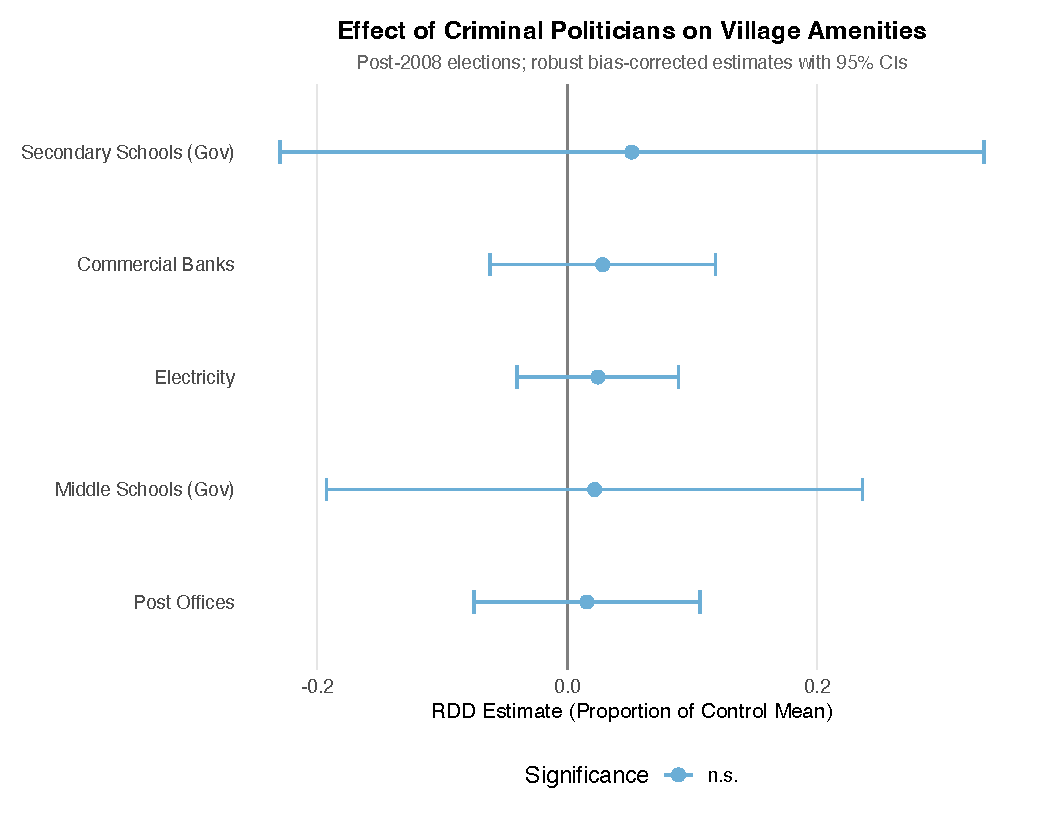
\includegraphics[width=0.85\textwidth]{figures/fig_mechanism_decomposition.pdf}
\caption{RDD Estimates for Village Amenity Outcomes}
\label{fig:mechanism_full}
\begin{minipage}{0.85\textwidth}
\small \textit{Notes:} Point estimates and 95\% confidence intervals for the effect of electing a criminal politician on 2011 village amenity levels (controlling for 2001 baselines). Coefficients expressed as share of the control-group mean. Color indicates statistical significance.
\end{minipage}
\end{figure}

% Figure promoted to main text as fig:cov_balance_main

\begin{figure}[H]
\centering

\includegraphics[width=0.85\textwidth]{figures/fig_placebo.pdf}
\caption{Placebo Cutoff Estimates}
\label{fig:placebo}
\begin{minipage}{0.85\textwidth}
\small \textit{Notes:} Point estimates and 95\% confidence intervals for the RDD at false cutoffs $\{-15, -10, -5, 0, +5, +10, +15\}$. The true cutoff (0) estimate is highlighted. All specifications include covariates.
\end{minipage}
\end{figure}

\begin{figure}[H]
\centering

\includegraphics[width=0.85\textwidth]{figures/fig_heterogeneity.pdf}
\caption{Heterogeneity: Nightlights Growth by Subgroup}
\label{fig:heterogeneity_full}
\begin{minipage}{0.85\textwidth}
\small \textit{Notes:} RDD estimates for nightlights growth in subsamples. BIMARU states: Bihar, Madhya Pradesh, Rajasthan, Uttar Pradesh (including successor states). Point estimates with 95\% bias-corrected robust confidence intervals.
\end{minipage}
\end{figure}

\begin{table}[H]
\centering
\caption{RDD Sample: Distribution of Close Races}
\label{tab:close_races}
\begin{threeparttable}
\begin{tabular}{lcc}
\toprule
Margin range & Number of elections & Cumulative \\
\midrule
$|M| \leq 1\%$ & 204 & 204 \\
$1\% < |M| \leq 2\%$ & 197 & 401 \\
$2\% < |M| \leq 3\%$ & 191 & 592 \\
$3\% < |M| \leq 5\%$ & 382 & 974 \\
$5\% < |M| \leq 10\%$ & 804 & 1,778 \\
$10\% < |M| \leq 20\%$ & 892 & 2,670 \\
$|M| > 20\%$ & 579 & 3,249 \\
\bottomrule
\end{tabular}
\begin{tablenotes}[flushleft]
\small
\item \textit{Notes:} Distribution of the running variable (criminal minus non-criminal vote margin) in absolute value across the full RDD sample of 3,249 elections.
\end{tablenotes}
\end{threeparttable}
\end{table}

\end{document}
